%!TEX TS-program = xelatex
\documentclass[main]{subfiles}
%这是一个子文件,单独编译时会自动导入main文件的导言区
%这里可以放自定义命令,不会和别人的冲突请放心
%但是不能放newtheorem等高级命令,需要请在群里说
%下面是一些数学命令的简化,可以保留,可以删去,也可以按你的习惯修改
\newcommand{\mx}{\mathrm{d}x}
\newcommand{\my}{\mathrm{d}y}
\newcommand{\mz}{\mathrm{d}z}
\newcommand{\mr}{\mathrm{d}r}
\newcommand{\mmu}{\mathrm{d}u}
\newcommand{\mv}{\mathrm{d}v}
\newcommand{\mte}{\mathrm{d}\theta}
\newcommand{\mfai}{\mathrm{d}\varphi}
\newcommand{\df}{\dfrac}
\newcommand{\tf}{\tfrac}
\newcommand{\pa}{\partial}
\newcommand{\di}{\displaystyle}
\newcommand{\q}{$}
\newcommand{\bo}{\boldsymbol}
\newcommand{\te}{\theta}
\newcommand{\fai}{\varphi}
\newcommand{\cd}{\cdot}
\newcommand{\sq}{\sqrt}
\newcommand{\uns}{\underset}
\newcommand{\Om}{\Omega}
\newcommand{\ti}{\times}
\newcommand{\la}{\lambda}
\newcommand{\ora}{\overrightarrow}
\newcommand{\al}{\alpha}
\newcommand{\be}{\beta}
\newcommand{\ga}{\gamma}
\newcommand{\gt}{\geqslant}
\newcommand{\lt}{\leqslant}
\newcommand{\bs}{\boldsymbol}
\newcommand{\va}{\varepsilion}
\newcommand{\bb}{\mathbb}

\begin{document}
\renewcommand{\filename}{subfile23}%在这里填你的文件名,避免\label冲突
%这里开始写你的代码

%\title{}\renewcommand\maketitlehookc{\vspace{-18ex}}\date{}

%\maketitle
\section{正弦定理和余弦定理}

%In trigonometry, the law of sines, sine law, sine formula, 
%or sine rule is an equation relating the lengths of the sides of 
%any triangle to the sines of its angles. According to the law,

在三角学中,正弦定理是一个把三角形的边与角联系起来的定理,这定理表明:
$$
\frac{a}{\sin \alpha}=\frac{b}{\sin \beta}=\frac{c}{\sin \gamma}=2 R,
$$
这里 $a, b$ 和 $c$ 是三角形的边长,而 $\alpha, \beta$ 和 $\gamma$ 则分别是
三条边所对应的角. $R$ 是三角形外接圆半径.
当这式子的最后一部分不被使用时,该定理也被陈述为以下形式:
%where $a, b$, and $c$ are the lengths of the sides of a triangle, 
%and $\alpha, \beta$, and $\gamma$ are the opposite angles (see figure 2), 
%while $R$ is the radius of the triangle's circumcircle. 
%When the last part of the equation is not used, 
%the law is sometimes stated using the reciprocals;

$$
\frac{\sin \alpha}{a}=\frac{\sin \beta}{b}=\frac{\sin \gamma}{c} .
$$

%The law of sines can be used to compute the remaining sides of a triangle when two angles and a side are known-a technique known as triangulation. It can also be used when two sides and one of the non-enclosed angles are known. In some such cases, the triangle is not uniquely determined by this data (called the ambiguous case) and the technique gives two possible values for the enclosed angle.

%The law of sines is one of two trigonometric equations commonly applied to find lengths and angles in scalene triangles, with the other being the law of cosines.

%The law of sines can be generalized to higher dimensions on surfaces with constant curvature.
当两个角度和一条边已知时,正弦定理可用于计算三角形的剩余边,这种技术称为三角测量. 

\iffalse
\begin{proof}
  The area of any triangle can be written as one half of its base times its height. Selecting one side of the triangle as the base, the height of the triangle relative to that base is computed as the length of another side times the sine of the angle between the chosen side and the base. Thus depending on the selection of the base, the area $T$ of the triangle can be written as any of:
$$
T=\frac{1}{2} b(c \sin \alpha)=\frac{1}{2} c(a \sin \beta)=\frac{1}{2} a(b \sin \gamma) .
$$

Multiplying these by $\frac{2}{a b c}$ gives
$$
\frac{2 T}{a b c}=\frac{\sin \alpha}{a}=\frac{\sin \beta}{b}=\frac{\sin \gamma}{c} .
$$

As shown in the figure, let there be a circle with inscribed $\triangle A B C$ and another inscribed $\triangle A D B$ that passes through the circle's center $\mathbf{O}$. The $\angle A O D$ has a central angle of $180^{\circ}$ and thus $\angle A B D=90^{\circ}$, by Thales's theorem. Since $\triangle A B D$ is a right triangle,
$$
\sin \delta=\frac{\text { opposite }}{\text { hypotenuse }}=\frac{c}{2 R},
$$
where $R=\frac{d}{2}$ is the radius of the circumscribing circle of the triangle. ${ }^{[9]}$ Angles $\gamma$ and $\delta$ have the same central angle thus they are the same, by the inscribed angle theorem: $\gamma=\delta$. Therefore,
$$
\sin \delta=\sin \gamma=\frac{c}{2 R} .
$$

Rearranging yields
$$
2 R=\frac{c}{\sin \gamma}
$$

Repeating the process of creating $\triangle A D B$ with other points gives
$$
\frac{a}{\sin \alpha}=\frac{b}{\sin \beta}=\frac{c}{\sin \gamma}=2 R .
$$
\end{proof}
\fi
\begin{figure}[H]
 
  \centering
      
      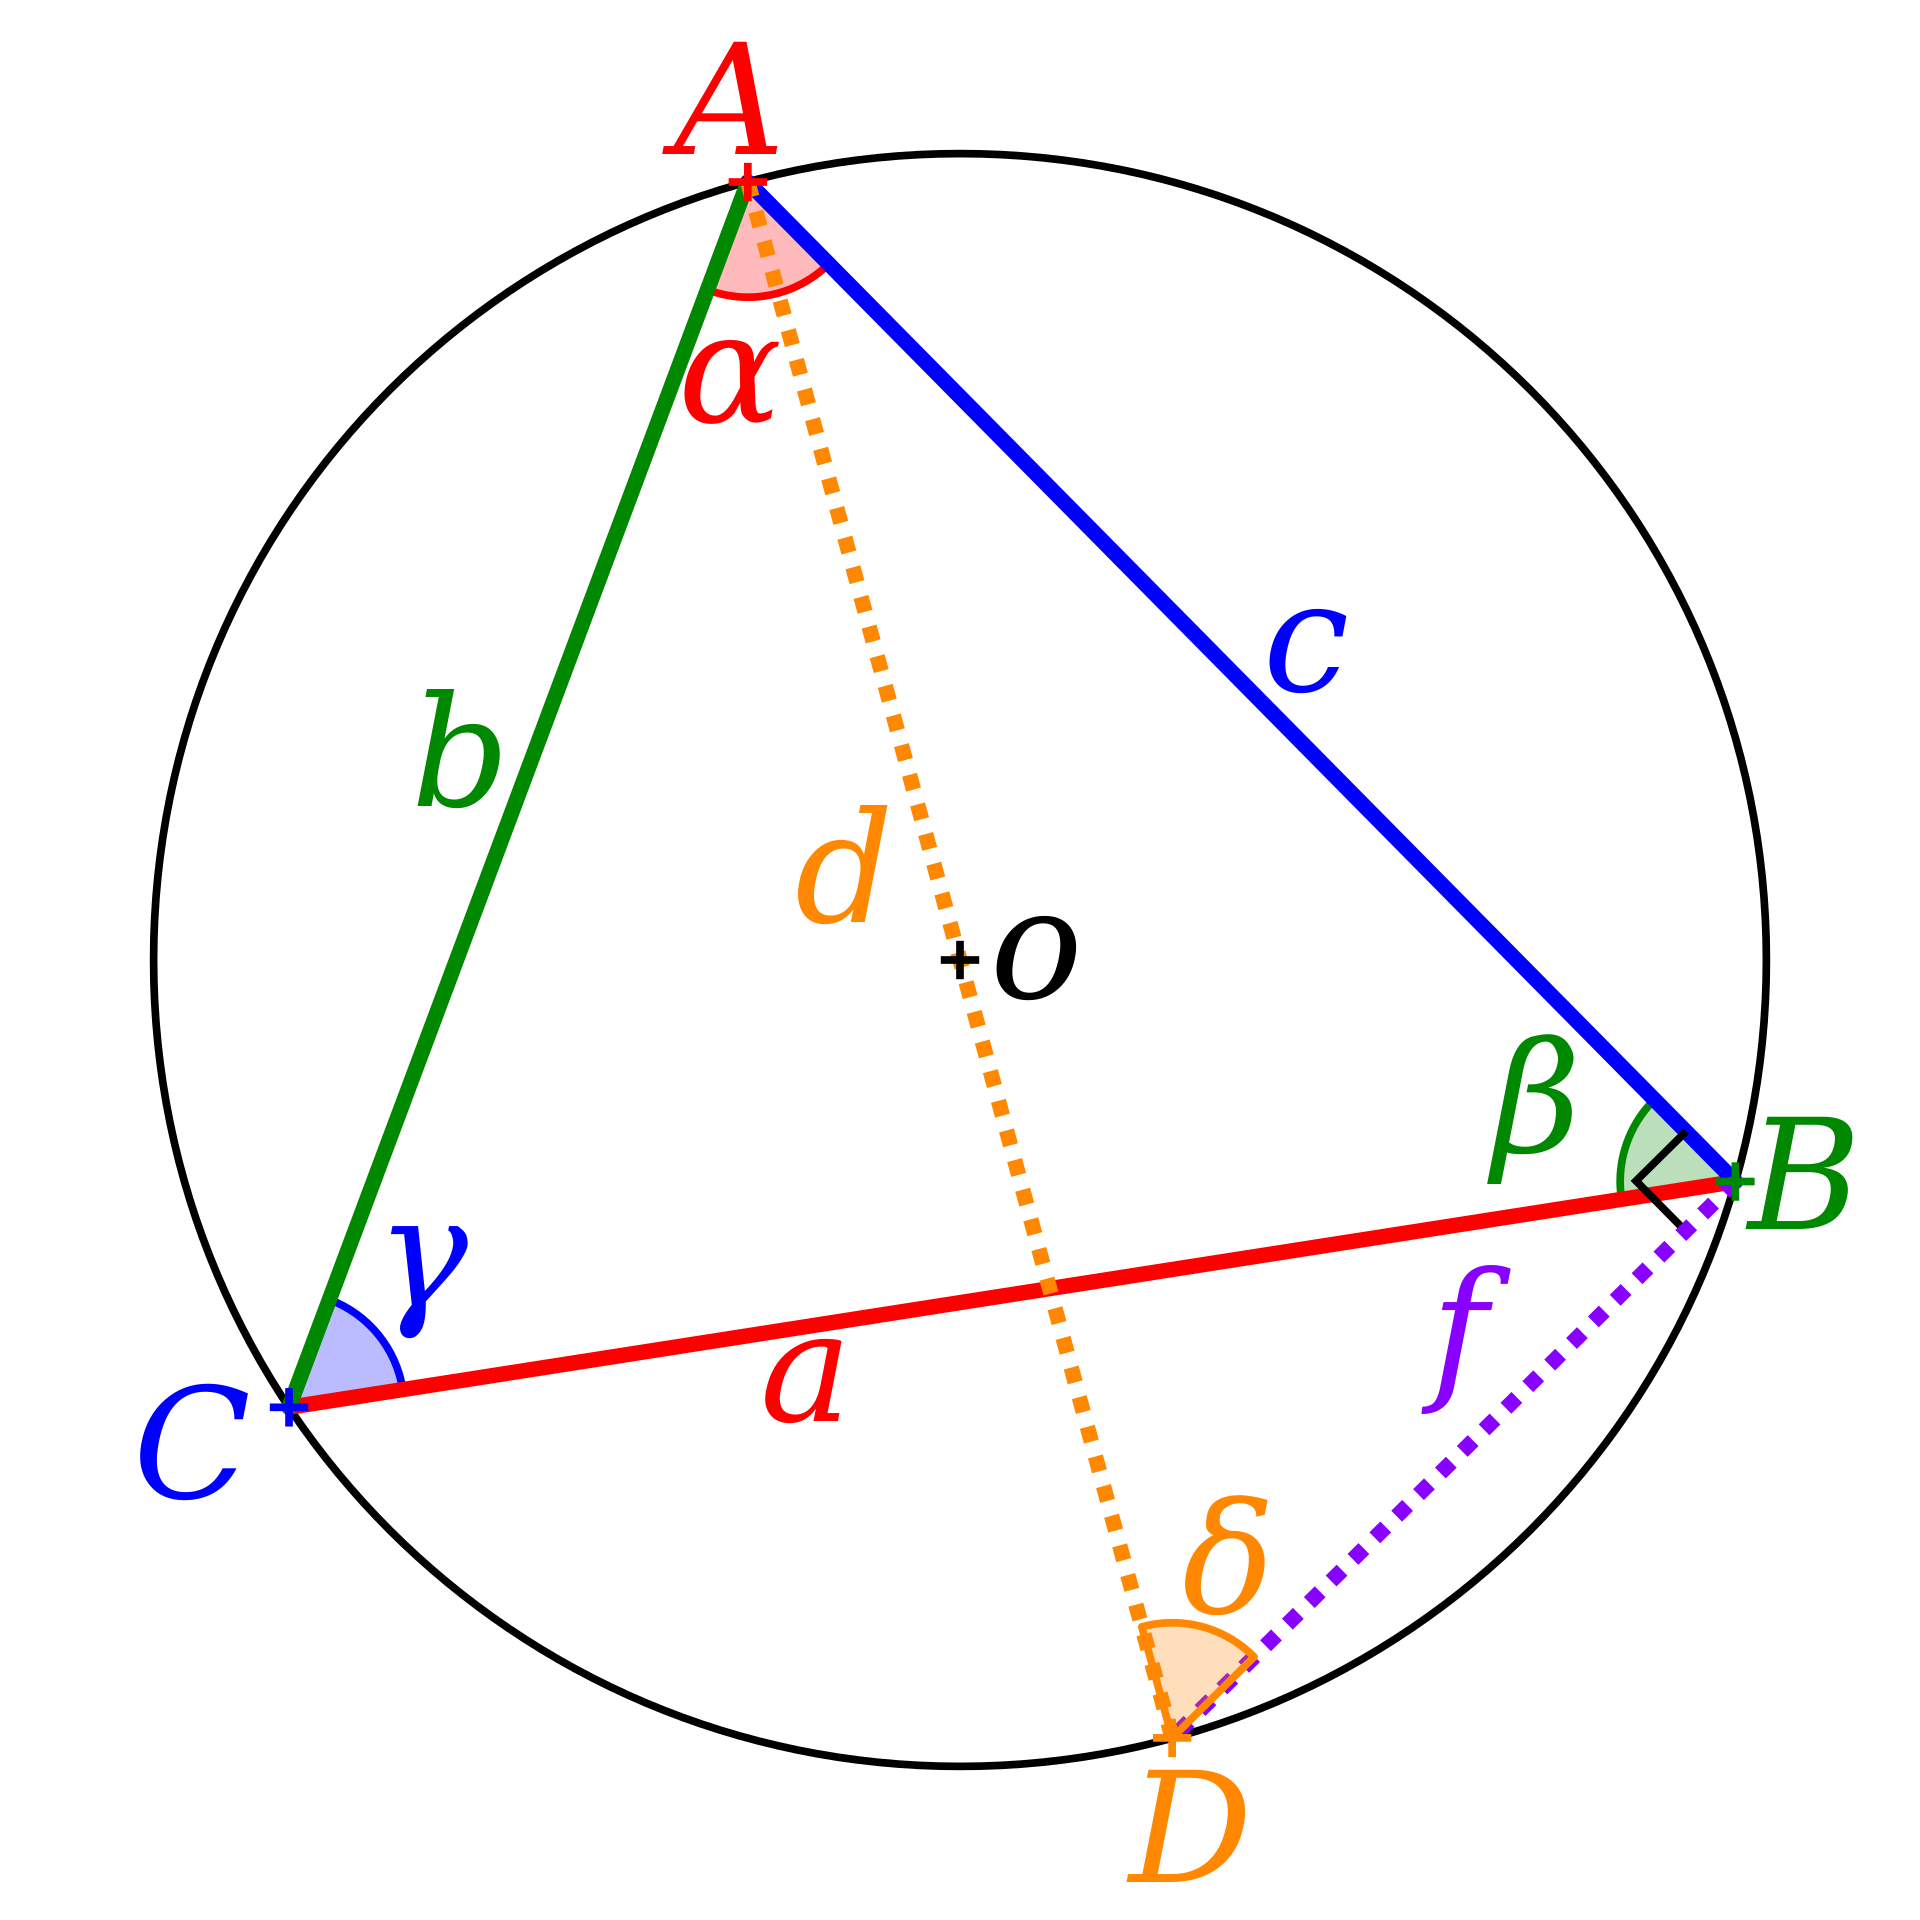
\includegraphics[width=0.30\textwidth]{zxdl.png}
       %\caption{}
  
  \end{figure}
  
%In trigonometry, the law of cosines (also known as the cosine formula or cosine rule) relates the lengths of the sides of a triangle to the cosine of one of its angles. For a triangle with sides $a, b$, and $c$, opposite respective angles $\alpha, \beta$, and $\gamma$ (see Fig. 1), the law of cosines states:
在三角学中,余弦定理涉及
三角形的边长与其一个角的余弦值.余弦定理指出:
$$
\begin{aligned}
& c^2=a^2+b^2-2 a b \cos \gamma, \\
& a^2=b^2+c^2-2 b c \cos \alpha, \\
& b^2=a^2+c^2-2 a c \cos \beta .
\end{aligned}
$$
这里 $a, b$ 和 $c$ 是三角形的边长,而 $\alpha, \beta$ 和 $\gamma$ 则分别是
三条边所对应的角.

余弦定理涵盖了勾股定理.
如果 $\gamma$ 是直角,则 $\cos\gamma = 0$,余弦定律变化为 $c^2 = a^2 + b^2$,这就是勾股定理.

%The law of cosines generalizes the Pythagorean theorem, which holds only for right triangles: if $\gamma$ is a right angle then $\cos \gamma=0$, and the law of cosines reduces to $c^2=a^2+b^2$.
%Consider a triangle with sides of length a, b, c, 
%where θ is the measurement of the angle opposite the side of length c. 
%This triangle can be placed on the Cartesian coordinate 
%system with side a aligned along the x axis and angle θ placed at the
%origin, by plotting the components of the 3 points of the triangle 
%as shown in Fig. 4:
如果我们设边 $c$ 所对应的角为 $\theta$,把三角形放在笛卡尔坐标系中,将 $BC$ 边
放在 $x$ 轴上,顶点 $C$ 与坐标原点重合,那么点 $A,B,C$ 的坐标即为
$$
\begin{aligned}
  A=(b\cos \theta ,b\sin \theta ),
B=(a,0),{\text{ and }}C=(0,0).
\end{aligned}
$$
由距离公式:
$$
\begin{aligned}
  c={\sqrt {(a-b\cos \theta )^{2}+(0-b\sin \theta )^{2}}}.
\end{aligned}
$$
将式子两边平方并化简:
$$
\begin{aligned}
  c^{2}&=(a-b\cos \theta )^{2}+
  (-b\sin \theta )^{2}\\&=a^{2}-2ab\cos \theta +b^{2}
  \cos ^{2}\theta +b^{2}\sin ^{2}\theta \\&=a^{2}+b^{2}
  (\sin ^{2}\theta +\cos ^{2}\theta )-2ab\cos \theta \\
  &=a^{2}+b^{2}-2ab\cos \theta .
\end{aligned}
$$
这个证明的一个优点在于它不需要分情况考虑三角形是否是锐角、直角或钝角.
%  An advantage of this proof is that it does not require the consideration 
%of different cases for when the triangle is acute, right, or obtuse.
\end{document}
